% LaTeX Template
\RequirePackage{ifluatex}
\ifluatex
  \documentclass[a4j,10ptj,fleqn]{ltjsbook}  % LuaLaTeX
\else
  \documentclass[uplatex,a4j,twoside,fleqn]{jsbook}  % upLaTeX
\fi

\usepackage{ifthen}
\newcommand{\thesistype}{doctor}  % 博士論文
% \newcommand{\thesistype}{master}  % 修士論文
% \newcommand{\thesistype}{bachelor}  % 卒業論文
\ifluatex
  \usepackage{graphicx, xcolor}
  \usepackage{luatexja-otf}
  \usepackage{luatexja-fontspec}
  \usepackage[ms]{luatexja-preset}
  \setmainfont[Ligatures=TeX]{Times New Roman}
\else
  \usepackage[dvipdfmx]{graphicx, xcolor}
\fi
\usepackage[intlimits]{amsmath}
\usepackage{newtxtext, newtxmath}
\usepackage{mathrsfs}  % \mathscr用
\usepackage{booktabs}  % 綺麗な表組み
\usepackage{multirow}  % 複数行や複数列の表組み
\usepackage{type1cm}  % フォント拡大縮小
\usepackage{scalefnt}  % フォント拡大縮小
\usepackage{fancyhdr}  % ヘッダーに罫線を引く
\usepackage{comment}  % 複数行のコメントアウト
\usepackage{subfigure}  % 図を複数並べる
% \usepackage[notref,notcite]{showkeys} % ラベル表示 (提出前にコメントアウト)

\usepackage[nocolsep]{dotseqn}  % 数式を点線で結ぶ
\makeatletter
\renewcommand\EqnDots{\leaders\hbox{\kern1\p@ .\kern1\p@}\hfill}
\makeatother
\renewcommand{\textbf}[1]{{\bfseries\sffamily#1}}  %太字にする際ゴシック体とセリフ体とを区別なく太くする

\usepackage{jsbook2thesisL}

% citation
\usepackage{overcite}
\renewcommand\citeform[1]{(#1)}

% 速度vに関するフォント定義(体積vと区別)
% \newcommand{\sv}{\mbox{\usefont{T1}{cmr}{m}{it}{v}}}  % Scalar v
% \newcommand{\vv}{\mbox{\usefont{T1}{cmr}{bx}{it}{v}}}  % Vector v

% 明朝体での半角括弧(機械学会準拠)
% \newcommand*{\parentheses}[1]{{\mc (}{#1}{\mc )}}

% 栞
\ifluatex
\usepackage[unicode=true,bookmarks=true, %
  colorlinks=true,linkcolor=black,citecolor=black, %
  bookmarksnumbered=true]{hyperref}
\else
\usepackage[dvipdfm,bookmarks=true,colorlinks=true,%%
    linkcolor=black,citecolor=black,
    bookmarksnumbered=true,bookmarkstype=toc
    ]%%
    {hyperref}
\usepackage{pxjahyper}
\fi

% 索引
\usepackage{makeidx}
\makeindex

\usepackage{lipsum}  % ダミーテキスト用

% 文書
\begin{document}
% title
\ifthenelse{\equal{\thesistype}{doctor}}{%
  % 博士論文記入用フォーマット
\begin{titlepage}
    \begin{center}
        {\LARGE 学位論文 博士(工学)}\\
        \vspace{3cm}
        {\LARGE 〇〇〇〇〇〇〇〇〇〇} \\[5mm]
        {\LARGE 〇〇〇〇〇〇〇〇〇〇} \\[5mm]
        {\LARGE 〇〇〇〇〇〇〇〇〇〇} \\
        \vspace{3cm}
        {\LARGE 20XX年度} \\
        \vspace{8cm}
        {\LARGE 〇〇大学大学院〇〇研究科} \\
        \vspace{2cm}
        {\LARGE 〇〇 〇〇} \\
    \end{center}
\end{titlepage}
    
}{}
\ifthenelse{\equal{\thesistype}{master}}{%
  % 修士論文記入用フォーマット
\begin{titlepage}
    {\LARGE 修士論文} \hspace{\fill} {\LARGE 20XX年度}
    \vspace{1.8cm}
    \begin{center}
         {\Huge 〇〇〇〇〇〇〇〇〇〇\\[2truemm]
         〇〇〇〇〇〇〇〇〇〇\\[2truemm]
         〇〇〇〇〇〇〇〇〇〇\\[4truemm]
         〇〇〇〇〇〇〇〇〇〇} \\
        \vspace{2cm}
        {\Huge 〇〇 〇〇} \\[1truemm]
        {\LARGE (学籍番号:11111111)} \\
        \vspace{5cm}
        {\LARGE 指導教員 教授 〇〇 〇〇} \\
        \vspace{3cm}
        {\Large 20XX年3月} \\
        \vspace{1cm}
        {\LARGE 〇〇大学大学院〇〇〇研究科} \\
        {\LARGE 〇〇工学専攻} \\
    \end{center}
\end{titlepage}

}{}
\ifthenelse{\equal{\thesistype}{bachelor}}{%
  % 卒業論文記入用フォーマット
\begin{titlepage}
    \begin{flushright}
        \Large XX-XX  % 論文番号
    \end{flushright}
    \vspace{2cm}
    \begin{center}
        {\LARGE 20XX年度卒業論文} \\
        \vspace{2cm}
        {\LARGE 〇〇〇〇〇〇〇〇〇〇\\[2truemm]
        〇〇〇〇〇〇〇〇〇〇\\[2truemm]
        〇〇〇〇〇〇〇〇〇〇\\[4truemm]
        〇〇〇〇〇〇〇〇〇〇} \\

        \vspace{4.5cm}
        {\LARGE 指導教員 〇〇〇〇 教授} \\
        \vspace{1cm}
        {\LARGE 〇〇大学 〇〇学部 〇〇学科} \\
        \vspace{2cm}
        {\LARGE 学籍番号 11111111} \\
        \vspace{1cm}
        {\LARGE 〇〇 〇〇} \\
    \end{center}
\end{titlepage}

}{}
\mbox{} \thispagestyle{empty} \newpage  % 空白ページ挿入

% abstract
\ifthenelse{\equal{\thesistype}{master}}{%
  % 論文要旨(和文)
\newpage
\pagestyle{empty}
\begin{center}
{\scalefont{2}論文要旨} \\
\vspace{1cm}
{\scalefont{1.6} 〇〇〇〇〇〇〇〇〇〇} \\
\vspace{0.2cm}
{\scalefont{1.6} 〇〇〇〇〇〇〇〇〇〇} \\
\vspace{0.2cm}
{\scalefont{1.6} 〇〇〇〇〇〇〇〇〇〇} \\
\end{center}
\vspace{0.5cm}
{\large 
 本研究では,
} \\
  % 要旨(和文)
  % 論文要旨(英文)
\newpage
\pagestyle{empty}
\begin{center}
{\scalefont{2} Thesis Abstract} \\
\vspace{1cm}
{\scalefont{1.6} 〇〇〇〇〇〇〇〇〇〇} \\
\vspace{0.1cm}
{\scalefont{1.6} 〇〇〇〇〇〇〇〇〇〇} \\
\vspace{0.1cm}
{\scalefont{1.6} 〇〇〇〇〇〇〇〇〇〇} \\
\end{center}
\vspace{0.5cm}
{\large 
\hspace{5ex} In this thesis,
}\\
\newpage
  % 要旨(英文)
  \newpage
}{}

% 目次
%\pagenumbering{roman}
\frontmatter
\tableofcontents  % 目次出力
\newpage

% fancy設定
\pagestyle{fancy}
\fancyhf{}
\fancyhead[RE,LO]{\thepage}
\fancyhead[LE]{\nouppercase{\rightmark}}
\fancyhead[RO]{\nouppercase{\leftmark}}
\fancyhead[LE,RO]{\thepage}	 % 偶数ページは左に,奇数ページは右にページ番号を出力
\fancyhead[RE]{\nouppercase{\leftmark}}	 % 偶数ページに\markleftで定義した文字を出力
\fancyhead[LO]{\nouppercase{\rightmark}}  % 奇数ページに\markrightで定義した文字を出力
\fancypagestyle{plainfoot}{  %
  \fancyhf{}  % remove everything
  %\renewcommand{\chaptermark}[1]{\markboth{第\thechapter章 \, #1}{}}
  %\renewcommand{\sectionmark}[1]{\markright{#1}{}}
}

% 本文
\mainmatter
\chapter{緒言}
\label{ch_preface}
\markboth{\ref{ch_preface}.緒言}{\ref{ch_preface}.緒言}

\section{本研究の背景}
\label{preface_background}
Burgersベクトル\index{ばーがーすべくとる@Burgersベクトル}は,現配置において式\eqref{eq_bergers_vector}で表される~\cite{kondo1955non-riemannian}.
%
\begin{equation}
  \label{eq_bergers_vector}
    \tilde{B}{}^{a}
    = -\int_{\mathscr{S}} \left[ \hat{T}{}^{..a}_{bc} + \frac{1}{2} C^{\ell{}-1ae}
      \left( \hat{R}{}_{bc[de]} + \hat{R}{}_{bc(de)} \right) x^{d} \right] \mathrm{d} x^{b} \wedge \mathrm{d} x^{c}
  \dotfill
\end{equation}
%
これを図示すると,図\ref{fig_paper_irasutoya}のようになる.
%
\begin{figure}[bp]
    \centering
    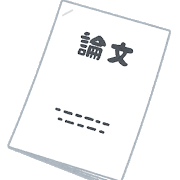
\includegraphics{./figure/document_ronbun_taba.png}
    \caption{Paper.}
    \label{fig_paper_irasutoya}
\end{figure}
%
  % 緒言

% 謝辞
\chapter*{謝辞}
\addcontentsline{toc}{chapter}{謝辞}
\markboth{謝辞}{謝辞}

本研究は,著者が〇〇大学大学院〇〇〇研究科〇〇〇専攻在籍中に,〇〇〇〇教授の御指導の下で行ったものであり,現在に至るまでの長きに渡る研究生活において同教授より賜りました熱心な御指導,御鞭撻に対して厚く御礼申し上げます.

\vspace{\baselineskip}
\hspace{5truemm}
20XX年XX月
\hspace{10truemm}
〇〇〇〇
\hspace{10truemm}
著者 〇〇 〇〇


% 参考文献
\bibliographystyle{./chap/sjunsrt_d.bst}
\bibliography{./chap/reference.bib}

% 業績リスト
\ifthenelse{\equal{\thesistype}{doctor}}{%
  \chapter*{本研究に関する原著論文および口頭発表}
\addcontentsline{toc}{chapter}{本研究に関する原著論文および口頭発表}
\markboth{本研究に関する原著論文および口頭発表}{本研究に関する原著論文および口頭発表}

\section*{1.定期刊行誌掲載論文(主論文に関連する原著論文)}
\addcontentsline{toc}{section}{1.定期刊行誌掲載論文(主論文に関連する原著論文)}
なし.

\section*{2.定期刊行誌掲載論文(その他の論文)}
\addcontentsline{toc}{section}{2.定期刊行誌掲載論文(その他の論文)}
なし.

\section*{3.国際会議論文(査読付きのfull-length papers)}
\addcontentsline{toc}{section}{3.国際会議論文(査読付きのfull-length papers)}
なし.

\section*{4.その他の国際会議発表}
\addcontentsline{toc}{section}{4.その他の国際会議発表}
なし.

\section*{5.国内学会発表}
\addcontentsline{toc}{section}{5.国内学会発表}
なし.

}{%else
  \chapter*{学会講演目録}
\addcontentsline{toc}{chapter}{学会講演目録}

\begin{enumerate}
\renewcommand{\labelenumi}{(\arabic{enumi})}
\item
\underline{〇〇〇〇}*, 〇〇〇〇, ``〇〇〇〇〇〇〇〇〇〇'', 〇〇学会第XX回〇〇〇〇講演会論文集, No.XX-XX, (20XX-XX), XXXX, (X pages), 北海道. 
\end{enumerate}

}

% 補足
\appendix
\chapter{第\ref{ch_preface}章の補足}
\label{app_preface}
\markboth{補足\ref{app_preface}}{第\ref{ch_preface}章の補足}

\section{あああ}
あああ.


% 索引
%\printindex

\end{document}
